\section{Statistical estimation for unbiased evaluation}
\label{sec:method}

We will now formalize the problem of combining human evaluation with an automatic metric.
Let $\sX$ be a set of inputs (e.g., articles),
and let $S$ be the \emph{system} (e.g.\ for summarization),
which takes $x \in \sX$ and returns output $S(x)$ (e.g.\ a summary).
Let $\sZ = \{ (x, S(x)) : x \in \sX \}$ be the set of system predictions.
Let $Y(z)$ be the random variable representing the human judgment according to some evaluation prompt (e.g.\ grammaticality or correctness),
and define $f(z) = \E[Y(z)]$ to be the (unknown) \emph{human metric} corresponding to averaging over an infinite number of human judgments.
Our goal is to estimate the average across all examples:
\begin{align}
\mu \eqdef \E_z[f(z)] = \inv{|\sZ|} \sum_{z \in \sZ} f(z)
\end{align}
with as few queries to $Y$ as possible.

Let $g$ be an automatic metric (e.g. ROUGE), which maps $z$ to a real number.
We assume evaluating $g(z)$ is free.
The central question is how to use $g$ in conjunction with calls to $Y$ to produce an unbiased estimate $\hat\mu$ (that is, $\E[\hat\mu] = \mu$).
In this section, we will construct a simple estimator based on control variates~\citep{ripley2009stochastic},
and prove that it is minimax optimal.

%In many settings, sampling from $Y(z)$ costs resources (e.g. paying annotators) so we wish to minimize the number of queries to $Y(z)$.
%On the other hand, we would like a good estimate of $\mu_Y$, which fundamentally requires queries.
%We hope to gain in data efficiency by using an automatic metric that is correlated with the mean human response.
%The naive empirical mean only uses samples from $Y(z)$, while we provide a
%control variates estimator that both uses the samples from $Y(z)$ and the
%associated free-to-compute $g(z)$ values. Our estimator is both surprisingly
%simple and minimax optimal.

%In this work, we study the problem of estimating the mean human score of a particular system with the aid of an automatic metric that is correlated with the mean score. 

%In fact, under an uncorrelated human response assumption (not necessarily independent or identically distributed) and a correlated automatic metric, we provide an unbiased estimator with the minimax optimal variance (among unbiased estimators).
%The estimator is surprisingly simple and easy to compute. The relative efficiency of the estimator is influenced by two key quantities: $\rho$, the correlation between the automatic metric and the human metric, and $\gamma$, the relative human response variance.

%For this work, our objective will be to have an unbiased estimate with a low variance with the lowest resource cost.

\subsection{Sample mean}

We warm up with the most basic unbiased estimate, the sample mean.
We sample $z^{(1)}, \dots, z^{(n)}$ independently with replacement from $\sZ$.
Then, we sample each human judgment $y^{(i)} = Y(z^{(i)})$ independently.\footnote{%
Note that this independence assumption isn't quite true in practice since we do not control who annotates our data.}
Define the estimator to be $\musimple = \frac{1}{n} \sum_{i=1}^n y^{(i)}$.
Note that $\musimple$ is unbiased ($\E[\musimple] = \mu$).

We can define $\sigma^2_f \eqdef \Var(f(z))$ as the variance of the human metric
and $\sigma^2_a \eqdef \E_z[\Var(Y(z))]$ as the variance of human judgment averaged over $\sZ$.
By the law of total variance, the variance of our estimator
is
\begin{align}
\label{eqn:varsimple}
\Var(\musimple) = \frac{1}{n} (\sigma^2_f + \sigma^2_a).
\end{align}
% PL: too much
%Furthermore, $\musimple$ has the minimax optimal
%variance among unbiased estimators that are functions of $\{y^{(i)}\}$.
% This is the typical way of estimating means and we will use it as the baseline in this work.
%\stm{proposition? reference? obvious? I could use this as a gentle warm-up for the later minimax proof arguments.}

\subsection{Control variates estimator}

% Intuition
Now let us see how an automatic metric $g$ can reduce variance.
If there is no annotator variance ($\sigma^2_a = 0$) so that $Y(z) = f(z)$,
we should expect the variance of $f(z)-g(z)$ to be lower than the variance of
$f(z)$, assuming $g$ is correlated with $f$---see \reffig{variance_reduction} for an illustration.

The actual control variates estimator needs to
handle noisy $Y(z)$ (i.e.\ $\sigma^2_a > 0$) and
guard against a $g(z)$ with low correlation.
% Actual estimator
Let us standardize $g$ to have zero mean and unit variance, because we have
assumed it is free to evaluate.
As before, let $z^{(1)}, \dots, z^{(n)}$ be independent samples from $\sZ$ and
draw $y^{(i)} = Y(z^{(i)})$ independently as well.
We define the \emph{control variates estimator} as
\begin{align}
\mucontrol = \frac{1}{n} \sum_{i=1}^n y^{(i)} - \alpha g(z^{(i)}),
\end{align}
where
\begin{align}
  \alpha \eqdef \Cov(f(z),g(z)).
\end{align}
Intuitively, we have averaged over $y^{(i)}$ to handle the noise introduced by $Y(z)$, and scaled $g(z)$ to prevent an uncorrelated automatic metric from introducing too much noise.

An important quantity governing the quality of an automatic metric $g$
is the correlation between $f(z)$ and $g(z)$ (recall that $g$ has unit variance):
\begin{align}
\rho \eqdef \frac{\alpha}{\sigma_f}.  % PL: remove \sigma_g = 1
\end{align}

\begin{figure}
\centering
  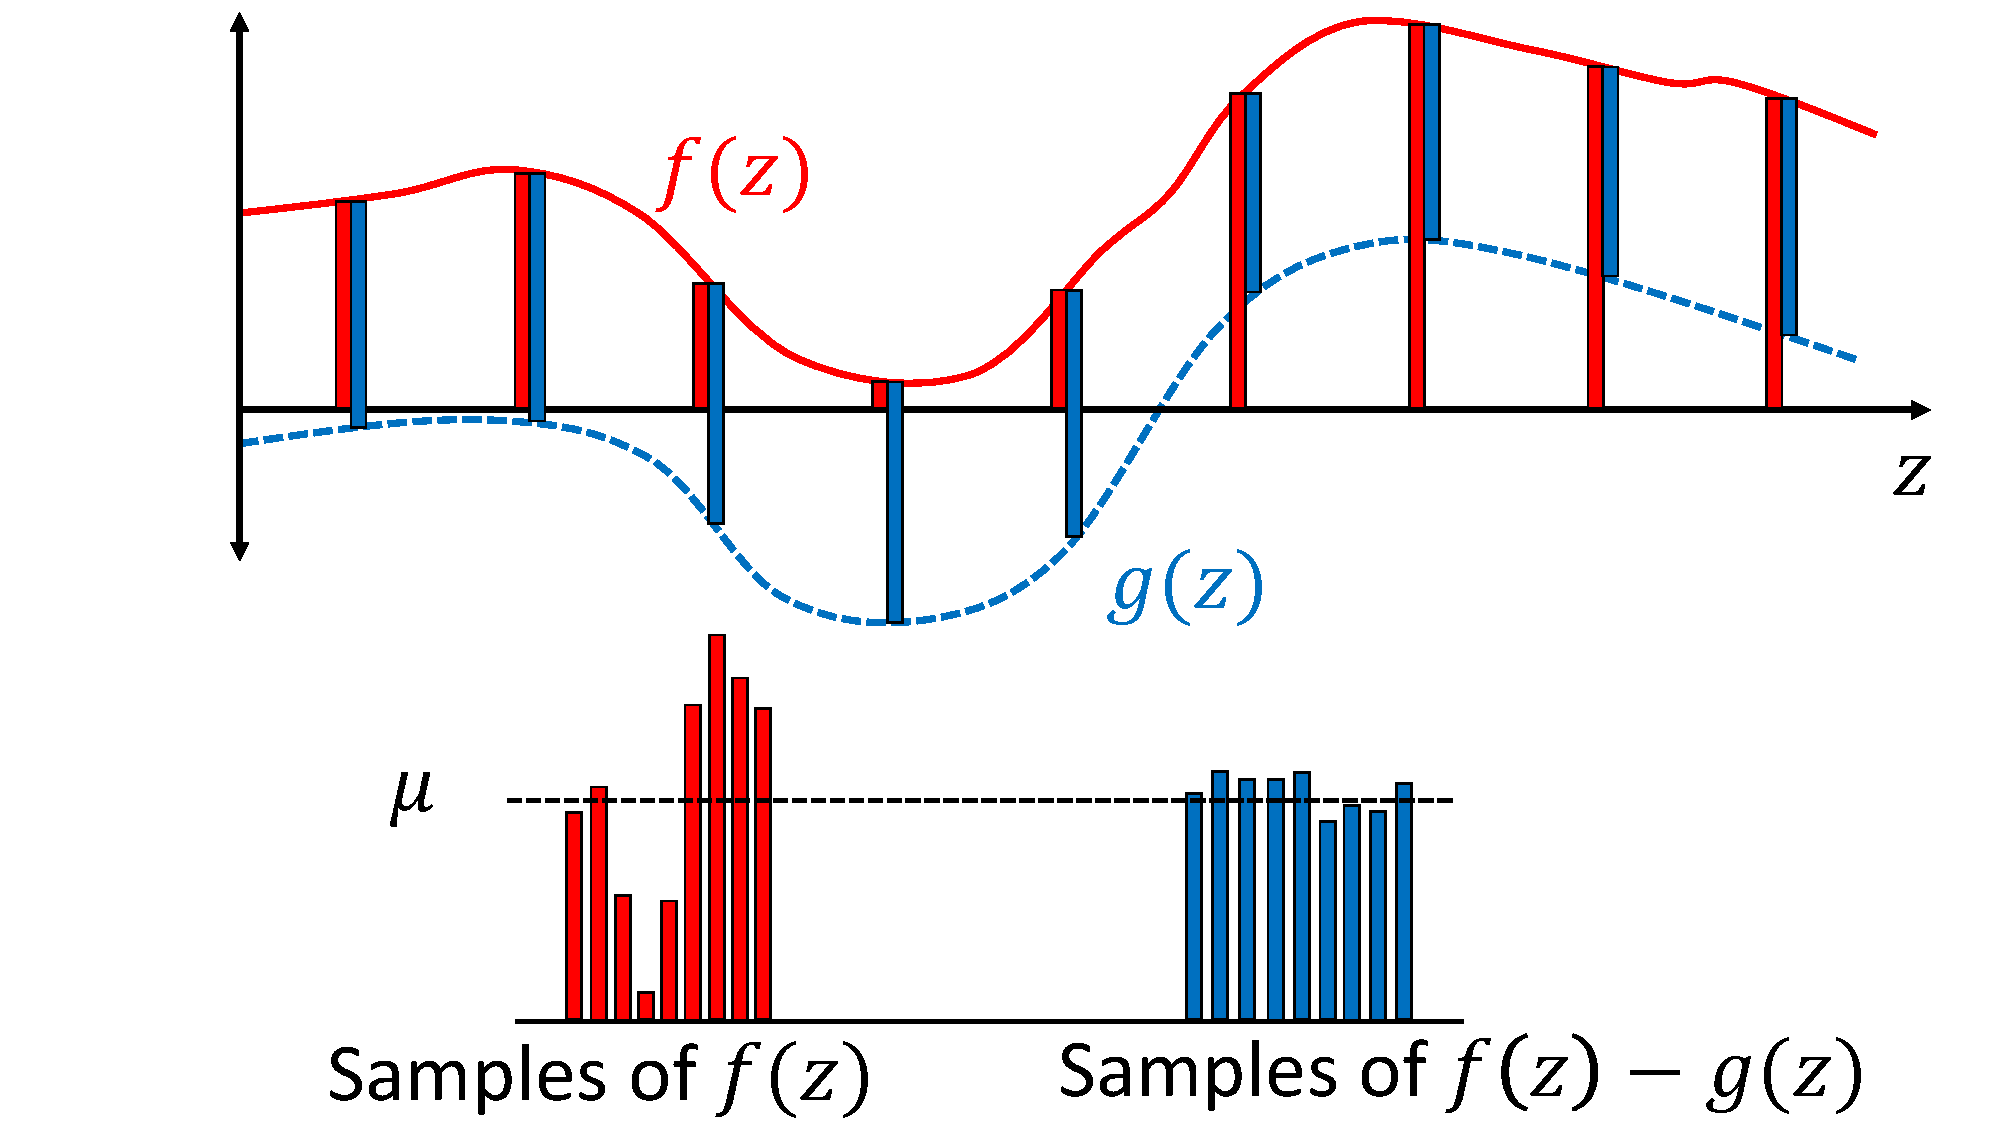
\includegraphics[width=\columnwidth]{figures/variance_reduction_extreme}
  \caption{\label{fig:variance_reduction}
  The samples from $f(z)$ have a higher variance than the samples
  from $f(z)-g(z)$ but the same mean. This is the key idea behind using control variates to reduce variance.}
\end{figure}

% Minimax optimal
We can show that among all distributions with
fixed $\sigma^2_f$, $\sigma^2_a$, and $\alpha$ (equivalently $\rho$), this estimator is minimax optimal, i.e.\ it has the least variance among all unbiased estimators:

\begin{theorem}
\label{thm:main}
Among all unbiased
  estimators that are functions of $y^{(i)}$ and $g(z^{(i)})$, and for all distributions with a given $\sigma^2_f$, $\sigma^2_a$, and $\alpha$,
\begin{align}
  \label{eqn:varcontrol}
  \Var(\mucontrol) = \frac{1}{n} (\sigma^2_f (1 - \rho^2) + \sigma^2_a),
\end{align}
and no other estimator has a lower worst-case variance.
\end{theorem}

%We typically will choose $n$ so that the sample variance is below some
%threshold.
%For both the empirical mean estimator and the control variates
%estimator, the variance goes as $\Theta(1/n)$ which means that the ratio of the
%sample complexities is the same as the ratio of the variances.
%Further, the
Comparing the variances of the two estimators (\refeqns{varsimple}{varcontrol}),
we define the \emph{data efficiency} as the ratio of the variances:
\begin{align}
\DE \eqdef \frac{\Var(\musimple)}{\Var(\mucontrol)} = \frac{1 + \gamma}{1-\rho^2 + \gamma},
\end{align}
where $\gamma \eqdef \sigma^2_a / \sigma^2_f$ is the normalized annotator variance.
Data efficiency is the key quantity in this paper:
  it is the multiplicative reduction in the number of samples required
  when using the control variates estimator $\mucontrol$ versus the sample mean $\musimple$.
Figure~\ref{fig:savings} shows the inverse data efficiency contours as a function of the correlation $\rho$
and $\gamma$.

\begin{figure}
\centering
  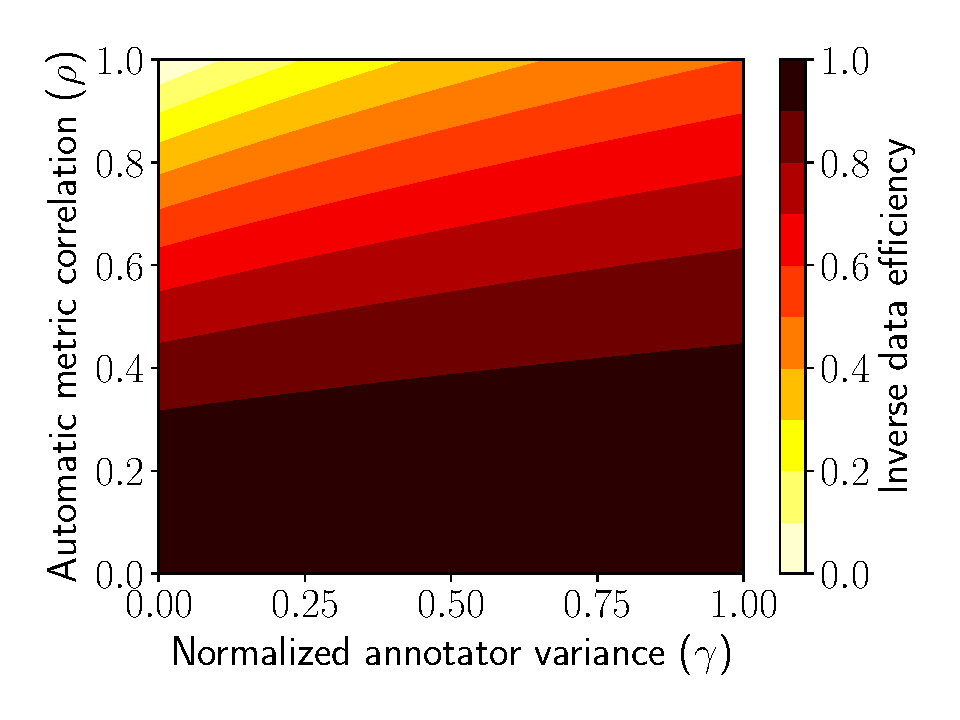
\includegraphics[width=\columnwidth]{figures/savings}
  \caption{\label{fig:savings} Inverse data efficiency for various values of
  $\gamma$ and $\rho$.  We need both low $\gamma$ and high $\rho$ to obtain
  significant gains.
  %Note that we do not even get a data efficiency of $2$ for
  %the darkest 5 stripes.
  % PL: removed it, if want to include it, need to explain better
  }
\end{figure}

When there is no correlation between human and automatic metrics ($\rho = 0$),
the data efficiency is naturally $1$ (no gain).
In order to achieve a data efficiency of
$2$ (half the labeling cost), we need $|\rho| \geq \sqrt{2}/2 \approx 0.707$.
Interestingly, even for an automatic metric with perfect correlation ($\rho=1$),
the data efficiency is still capped by $\frac{1 + \gamma}{\gamma}$:
unless $\gamma \to 0$ the data efficiency cannot increase unboundedly.
Intuitively, even
if we knew that $\rho=1$, $f(z)$ would be undetermined up to a
constant additive shift and just estimating the shift would incur a variance of $\frac{1}{n} \sigma_a^2$.
%\footnote{This is the case if the variance of $f$ at the single point is the average variance over all $z$.}

%At the same time, the higher the relative normalized annotator judgment variance $\gamma$, the worse
%the data efficiency gains.

%It is important to note that in order to use this estimator, we need to know
%the value of $\alpha = Cov(f(z),g(z))$. Later, we will show that estimating
%$\hat{\alpha}$ with the same sample introduces a bias and increase in variance
%that are low-order terms in $n$. However, the minimax optimal variance
%provides a lower bound in the cases where we don't know $\alpha$.

% $f(z)$ could be shifted In the case that $\rho=1$, $$f(z) - \mu_f = \frac{\sigma_f}{\sigma_g} (g(z) - \mu_g)$$ In the best case, when there exists a $z_0$ such that $g(z_0) = \mu_g$, $\mu_f = f(z_0)$. It seems like we would be done at this point, except that even to estimate $f(z_0)$ with $n$ samples incurs a variance of $\frac{1}{n} \sigma_a^2$ \footnote{this is only the case if the variance of $f$ at $z_0$ is the average variance overall all $z$}. Taking the ratio with the naive estimate yields the predicted $\frac{1 + \gamma}{\gamma}$.

\subsection{Using the control variates estimator}
The control variates estimator can be easily integrated into an existing evaluation:
we run human evaluation on a random sample of system outputs, automatic evaluation on all the system outputs, and plug in these results into \refalg{estimate}.

It is vital that we are able to evaluate the automatic metric on a significantly larger set of examples than those with human evaluations to reliably normalize $g(z)$:
without these additional examples, it be can shown that the optimal minimax estimator for $\mu$ is simply the naive estimate $\musimple$.
Intuitively, this is because estimating the mean of $g(z)$ incurs an equally large variance as estimating $\mu$.
In other words, $g(z)$ is only useful if we have additional information about $g$ beyond the samples $\{z^{(i)}\}$.

\refalg{estimate} shows the estimator.
In practice, we do not know $\alpha = \Cov(f(z),g(z))$, so we use a plug-in estimate $\hat{\alpha}$ in line 3 to compute the estimate $\widetilde{\mu}$ in line 4.
We note that estimating $\alpha$ from data does introduce a $O(1/n)$ bias,
but when compared to the standard deviation which decays as $\Theta(1/\sqrt{n})$, this bias quickly goes to $0$.
%Similarly, the variance is sub-optimal by a factor of only $1 + O(1/n)$.

\begin{proposition}
\label{prop:added_bias}
The estimator $\widetilde{\mu}$ in \refalg{estimate} has $O(1/n)$ bias.
\end{proposition}

\begin{algorithm}
      \caption{\label{alg:estimate}Control variates estimator}
      \begin{algorithmic}[1]
   \State{} {\bfseries Input:} $n$ human evaluations $y^{(i)}$ on system outputs $z^{(i)}$, \textit{normalized} automatic metric $g$ 
   \State{} $\overline{y} = \frac{1}{n} \sum_i y^{(i)}$
   \State{} $\hat{\alpha} = \frac{1}{n} \sum_i (y^{(i)} - \overline{y}) g(z^{(i)})$
   \State{} $\widetilde{\mu} = \frac{1}{n} \sum_i y^{(i)} - \hat{\alpha} g(z^{(i)})$
   \State{} {\bfseries return} $\widetilde{\mu}$
\end{algorithmic}
\end{algorithm}

An additional question that arises when applying \refalg{estimate} is figuring out how many samples $n$ to use.
Given a target variance, the number of samples can be estimated using \refeqn{varcontrol} with conservative estimates of $\sigma^2_f$, $\sigma^2_a$ and $\rho$.
Alternatively, our estimator can be combined with a dynamic stopping rule~\citep{mnih2008empirical} to stop data collection once we reach a target confidence interval.

\subsection{Discussion of assumptions}
We will soon see that empirical instantiations of $\gamma$ and $\rho$ lead to rather underwhelming data efficiencies in practice.
In light of our optimality result, does this mean there is no hope for gains?
%Modulo the asymptotically vanishing bias caused by estimating $\alpha$
%unfortunately, our theory states no other unbiased estimator with access to only human feedback and an automatic metric can do better.
Let us probe our assumptions.
We assumed that the human judgments are uncorrelated across different system outputs;
it is possible that a more accurate model of human annotators (e.g.\ \citet{passonneau2014benefits}) could offer improvements.
%\pl{really? isn't independent judgments the best we can hope for?}
% ^^ARUN: independent judgments are only the best choice under the naive model of human annotators we have which is that they are all interchangable and have iid noise. The intuition we have that turkers who label are lot are actually _better_ than those who label 1-2 examples is incongruent with  this simplistic model.
Perhaps with additional information about $g(z)$ such as calibrated confidence estimates,
we would be able to sample more adaptively.
Of course the most direct routes to improvement involve increasing the correlation of $g$ with human judgments and reducing annotator variance,
which we will discuss more later.

%our estimator is the minimax optimal over distributions with a fixed correlation between $f(z)$ and $g(z)$ and no further assumptions. 
%\ac{Reword.}

%\stm{The following sections will most likely be dropped, or briefly mentioned and moved to the appendix}

%\subsection{Arbitrary Annotators}
%\stm{Here we lay out the rigorous theoretical framework and prove optimality which suffices to prove the propositions above. We also find that the optimal experimental design is unique tasks and unique annotators, which matches our ``surrogate with noise'' section.}
%\subsubsection{Discrepancy with Algorithm}
%\stm{Here we talk about the sub-optimal variance introduced by not taking account of the annotators. It is small in practice.}

%\iffalse
%\subsection{Automatic metric without noise}
%
%Let us use the estimator
%
%$$\hat{\mu_f} = \frac{1}{n} \sum_i f(z^{(i)}) - \alpha g(z^{(i)})$$
%
%which has mean $\mu_f$ (unbiased) and variance,
%
%$$Var(\hat{\mu_f}) = \frac{1}{n}[ Var(f(z) - \alpha g(z))]$$
%$$ = \frac{1}{n}[\sigma^2_f - 2 \alpha Cov(f(z),g(z)) + \alpha^2]$$
%
%which is minimized when ${\alpha = Cov(f(z),g(z)) = \rho \sigma_f}$, for a final variance of
%
%$$Var(\hat{\mu_f}) = \frac{1}{n} \sigma^2_f (1 - \rho^2)$$
%
%In fact, this is the minimax optimal variance for an unbiased estimator.
%
%\begin{proposition}
%\label{prop:noiseless}
%In the noiseless setting where $Y_z = f(z)$, among all unbiased estimators, and among all distributions with fixed $\sigma^2_f$ and $Cov(f(z),g(z))$, the minimax variance is
%
%$$\frac{1}{n} \sigma^2_f (1 - \rho^2)$$
%
%\end{proposition}
%
%\fi
%%%%%%%%%%%%%%%%%%%%%%%%%%%%%%%
%%%%%%%%%%%%%%%%%%%%%%%%%%%%%%%
%%%%%%%%%%%%%%%%%%%%%%%%%%%%%%%
%\iffalse
%
%\paragraph{Problem definition.}
%Let us now formalize evaluation as an estimation problem:
%Let $S$ be the system we wish to evaluate on some defined \textit{metric} $f$ (e.g.\ accuracy, grammaticality, etc.) up to a given \textit{resolution} $\epsilon$ using a sufficiently large dataset of \textit{inputs} $X$.\footnote{%
%  A sufficiently large dataset is one that is big enough to evaluate any system to the target resolution $\epsilon$.}
%Let $z = (x, S(x))$ denote an input-output pair and let $Z$ be the set of \textit{input-output pairs} produced by $S$ on $X$: $Z \eqdef \{(x, S(x)) | x \in X \}$.
%Formally, our goal is to estimate $F \eqdef \E_{z \sim Z}[f(z)]$ to within $\epsilon$.
%
%In this paper, we look at ways to estimate $F$ given:
%\renewcommand{\labelenumi}{(\alph{enumi})}
%\begin{enumerate}
%  \item the ability to query a \textit{surrogate metric} (e.g.\ BLEU, ROUGE, a learned model, etc.) $g(z)$, and
%  \item the ability to query a human annotator $h(z)$ on a given example.
%\end{enumerate}
%Stated more formally, let $Z_A \subseteq Z$ be the subset of responses for which we have human annotations,
%$G = \{g(z) : z \in Z\}$ be the set of surrogate measurements \pl{notation is technically wrong because you don't want the image of $g$} and $H = \{h(z): z\in Z_A\}$ be the set of annotations obtained,
%then an estimator of $F$ is any function $\delta(G, H)$ such that $\E[\delta(G, H)] = F$, where the expectation is taken over the test set $X$ and the annotations $H$.
%
%\paragraph{Assumptions and constraints.}
%We make three key assumptions.
%\begin{enumerate}
%    \item Firstly, we assume that elements of the test set $X$ are independently drawn.
%    \item Secondly, we assume that annotators are independently assigned to examples.
%    \item Finally, we assume that the human responses $h(z)$ other than the fact that their mean accurately measures the ground truth, i.e.\ $\E[h(z)] = f(z)$. Alternatively, we consider that the metric $f(z)$ is \textit{defined} by the average human rating.
%      As a regularity condition, we assume that annotator noise: $\epsilon(z) \eqdef h(z) - f(z)$ has finite variance $\sigma^2_a < \infty$.
%    \pl{I think it's better to just \emph{define} the goal as measuring expectations over $h$;
%    removes a layer of indirection and an assumption
%    }
%\end{enumerate}
%We make no assumptions on the nature of interaction between annotator noise on different examples, as the noise might be correlated between two responses from the same annotator \pl{really? that seems like it would throw a wrench into variance calculations}.
%Likewise, we make no assumptions about $g(z)$ at all, and in particular, having seen the history of such automatic metrics in \refsec{setup}, we can expect that the correlation of $g(z)$ with $f(z)$ differs for across different systems. 
%
%Irrespective of the nature of the annotation noise and variation in surrogate correlation, we would like to ensure that $\E[\delta(G, H)] = F$ for any distribution of system outputs $Z$ and annotation noise $H$.
%In other words we would like the estimator to be \textit{unbiased}.
%For example, the constant estimator $\delta(G,H) = F_0$ will predict the correct result only when $F = F_0$ and be biased for every other possible $F$.
%\pl{what's $F_0$?}
%
%\pl{I'd defer as much of the above as possible to after you define the estimators;
%introduce only enough notation so that you can define the estimators;
%the analysis of variance should be a separate concern
%}
%
%\paragraph{Minimax optimal unbiased estimators.}
%
%Within the constraint of unbiased estimators, we would like to be able to find the one that has the least variance, ideally for any distribution of tests and annotators. 
%Unfortunately, for any particular distribution of tests and annotators its possible to construct an estimator $\delta$ that performs particularly well.
%In other words, except in certain circumstances (for example under the assumption that annotator noise is Gaussian), there is no uniformly minimum variance unbiased (UMVU) estimator. 
%Instead, we look for a minimax estimator: on that is guaranteed to have the least worst case variance:
%$\delta^* = \argmin_{\delta} \max_{X, H} \Var(\delta; X, H)$.
%
%\pl{I think the first thing you have to give is the naive estimator and the incorporating the model;
%'minimax' is going to scare people away
%}
%
%\paragraph{Model-free estimator.}
%
%As a baseline, let us first consider the case where we are trying to estimate $F$ without a model.
%In this case, because $h(z)$ is an unbiased predictor of $f(z)$, the estimator $\delta = \frac{1}{|Z_A|}\sum_{z \in Z_A} h(z)$ with a variance of at least $\frac{\sigma^2_f + \sigma^2_a}{n}$.
%
%\begin{figure}
%  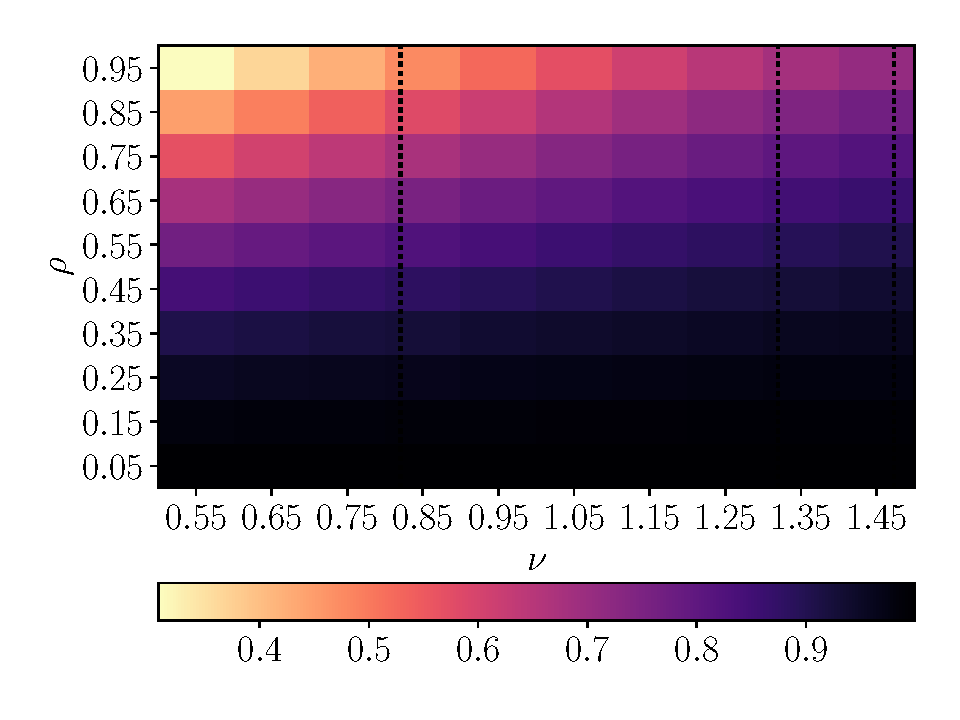
\includegraphics[width=\columnwidth]{figures/data_efficiency}
%  \caption{\label{fig:data-efficiency} The relative quantity of data that can be saved when using a model during evaluation, or data efficiency, depends on two fundamental quantities: normalized annotator variance $\nu = \sigma_a^2/\sigma_f^2$ and the model's correlation with the ground truth, $\rho$.
%  The plot above visualizes the dependence of data efficiency on $\nu$ and $\rho$.
%  The values of $\nu$ measured on our natural language evaluation benchmark is also highlighted: given the high levels of inter-annotator disagreement we find that the data efficiency is upper-bounded by 2 even on the most objective task in the benchmark, answer correctness on MSMarco. (TODO: make figure better)}
%\end{figure}
%
%\paragraph{Incorporating a model.}
%Let $g(z)$ be the evaluation model's estimate of $f(z)$. We study the following unbiased estimator:
%\[
%\Fh_g \eqdef \E_{Z}[g(z)] + \frac{1}{n}\sum_{i=1}^n f(z_i) - g(z_i).
%\]
%It is easy to verify that $\Fh_g$ is indeed an unbiased estimate of $F_S$.
%The variance of $\Fh_g$ is characterized as:
%\[
%\Var[\Fh_g] = \frac{\sigma_a^2 + (1-\rho^2)\sigma_f^2}{n},
%\]
%where $\rho$ is the Pearson correlation coefficient of $f$ and $g$, $\rho \eqdef \frac{\Cov[f(z)g(z)]}{\sigma_f \sigma_g}$.
%
%This analysis tells us two things, first that the variance of $\Fh_g$ is always less than that of $\Fh_a$ if $\rho > 0$ and secondly that the variance of $\Fh_a$ is bottlenecked by annotator variance $\sigma_a^2$: i.e. even a perfect model will incur some variance because of the annotator variance.
%
%\pl{In some sense, this is the core point, whereas currently, this is just another nested bullet}
%\pl{what happened to $h$?; do we need both $f$ and $h$?}
%
%\pl{talk about control variates and cite}
%
%\paragraph{Incorporating information about annotator identities}
%
%\pl{I think it might be better if we could defer this to another section;
%you want to quickly just get in, define the basic estimator, do a simple
%analysis, make your point; then do the annotator stuff as an extension;
%people are not going to have the patience to read the entire paper,
%so it should have a prefix property (news style): they should get the main point
%from begin to end on the basic version
%}
%
%First, we must define how the annotator labels $\fh_a(z)$ describe the ground truth.
%The most basic approach is to assume that each annotator produces an unbiased estimate of $f(z)$ with some i.i.d. noise:.
%Unfortunately, this model typically does not bear out in practice \pl{not worth even mentioning this as it's obvious that annotators have bias?}, as annotators often introduce some bias in their interpretation of the question. Instead, we assume that the set of all annotators as a whole do not introduce any bias to the task (even if any individual might). Such an approach leads us to define the following linear model:
%\[
%	\fh_a(z) = F_S + \delta f(z) + a + \epsilon,
%\]
%for some $z \in Z$.
%
%The variance of our estimate is characterized by 
%	the \textit{task variance} $\sigma^2_f \eqdef \sum_{z}[\delta f(z)^2]$,
%	\textit{annotator variance} $\sigma^2_a \eqdef \sum_{a}[a^2]$ and 
%	\textit{measurement variance} $\sigma^2_m \eqdef \sum[\epsilon^2]$.
%While task variance depends on the system at hand, the latter two quantities are more reflective of the evaluation setup.
%Of course, we would like there to be as little measurement variance $\sigma^2_m = 0$ as possible.
%
%Note that this formulation strictly subsumes the earlier model, where in $a = 0$ for every annotator and thus does not introduce any bias of its own.
%In this simpler model, we find that $\sigma^2_m \gets \sigma^2_a + \sigma^2_m$, increasing our measurement variance.
%
%In the sequel, we will find that the number of samples we need to estimate $F_S$ is dependent only on $\sigma_f^2$ and $\sigma_m^2$, and we can bound it using the latter.
%
%\paragraph{Incorporating surrogate confidences}
%
%\pl{same comment as above about deferring to later}
%
%Finally, we consider the scenario wherein we use the model's uncertainty to help guide which examples to annotate: presumably we will need fewer such annotations where the model is confident.
%Let $\epsilon_g(z)$ be the uncertainty reported by the model and let $\lambda_g$ be the degree of calibration of the model:
%\[
%\lambda_g \eqdef \E\left[ \left| |f(z) - g(z)| - \epsilon_g(z) \right| \right].
%\]
%
%In this setting, we use the following importance sampling estimator:
%\[
%	\Fh_c \eqdef \E[g(z)] + \sum_{i}^n \frac{p(z_i)}{q(z_i)} (f(z_i) - g(z_i)),
%\]
%where $z_i$ is drawn according to $q(z_i)$ and $p(z)$ is the uniform probability over $Z$.
%The variance of the estimator $\Fh_c$ depends on the distribution $q(z)$, but is minimized when $q(z) \propto p(z) |f(z) - g(z)|$.
%Assuming that our model's estimates are normally distributed around the true value $f(z)$, the expected value of $|f(z) - g(z)|$ is simply $\sqrt{\frac{2}{\pi}} \sigma_g(z)$.
%From this, we can estimate:
%\[
%\Var(\Fh_c) = \frac{\E[\sqrt{\sigma^2_a + \sigma^2_g(z)}]^2}{n}.
%\]
%Note that if the confidence estimates $\sigma^2_g(z)$ are uniform throughout, the expression for $\Var(\Fh_c)$ reduces to $\Var(\Fh_g)$, as expected. However, given a skew, we expect some gains.
%\fi
%
%% Formally define f(x) as what we want,
%%First, let $S$ be a system that produces some output $y \eqdef S(x)$ for a given input $x$.
%%Next, let $f(x, y)$ be the \textit{performance metric} we care about, e.g.\ correctness, grammaticality, etc.
%%Our goal is to estimate $F_S \eqdef \E_{\sX}[f(x, S(x))]$, where $x$ is sampled from set of possible inputs $\sX$.
%
%%In a typical classification setting, there is a single correct answer or label, $y^*$, for an input and $f(x,y)$ can be simply defined as accuracy: $f(x,y) = \I[y == y*]$.
%%When this is the case, $F_S$ is easy to estimate: we simply take the mean performance on a \textit{test set} $X$: $\Fh_S = \frac{1}{|X|} \sum_{x \in X} f(x, S(x))$.
%
%% g(x) as an automatic metric.
%%Unfortunately, in most generation contexts we do not have a single correct answer and we can not directly evaluate $f(x,y)$.
%%In our framework, we consider surrogate metrics (e.g.\ BLEU, ROUGE, ADEM, etc.) as an independent function $g(z)$ that is correlated with $f(z)$.
%%As we have seen in \refsec{setup}, in practice, $g(z)$ is only (weakly) correlated with $f(z)$ and its correlation varies depending on the system being evaluated.
%%% h(x) as annotation.
%%To correct for the biases introduced by the correlated metric, we also consider access to human annotations $h(z)$ which are related to $f(z)$ as follows: $h(z) \eqdef f(z) + \epsilon$, where $\epsilon$ is arbitrary zero-mean noise: in other words, $f(z) \eqdef \E[h(z)]$.
%%We make no assumptions on Gaussianity or independence.
%
%%For brevity, we will use $z = (x,y)$ to denote the input-output pair and $Z_S = \{(x, S(x)) : x \in X\}$ to be the set of input-output pairs generated by $S$.
%
%%Of course, because of inherent variation in the difficulty of task instances and performance of the system, we can only estimate the quality of the system up to a degree of \textit{precision} $\epsilon$ that primarily depends on the size of the dataset being evaluated.
%
%%\textbf{IMPORTANT: HOW DO WE ADDRESS THE FACT THAT OFTEN HUMAN judgmentS ARE REPORTED WITH SUPER HIGH VARIANCE! -- see \citet{snover2006ter} for example: they find HTER to have higher correlation than with 2 people!?!}
%
